\chapter{神经网络和反向传播算法}\label{chap:Bp}

\begin{introduction}
	\item 神经元~\ref{Bp:1}
	\item 神经网络是啥~\ref{Bp:2}
	\item 计算神经网络的输出~\ref{Bp:3}
	\item 神经网络的矩阵表示~\ref{Bp:4}
	\item 神经网络的训练~\ref{Bp:5}
	\item 反向传播算法~\ref{Bp:6}
	\item 反向传播算法的推导~\ref{Bp:7}
	\item 编程实战:神经网络的实现~\ref{Bp:8},\ref{Bp:12}
	\item 神经网络实战:手写数字识别~\ref{Bp:9}
	\item 超参数的确定~\ref{Bp:10}
	\item 模型的训练和评估~\ref{Bp:11}
	\item 向量化编程~\ref{Bp:13}
\end{introduction}

在上一篇文章中,我们已经掌握了机器学习的基本套路,对模型、目标函数、优化算法这些概念有了一定程度的理解,而且已经会训练单个的感知器或者线性单元了。在这篇文章中,我们将把这些单独的单元按照一定的规则相互连接在一起形成\textbf{神经网络},从而奇迹般的获得了强大的学习能力。我们还将介绍这种网络的训练算法:\textbf{反向传播算法}。最后,我们依然用代码实现一个神经网络。如果您能坚持到本文的结尾,将会看到我们用自己实现的神经网络去识别手写数字。现在请做好准备,您即将双手触及到深度学习的大门。


\section{神经元}\label{Bp:1}

神经元和感知器本质上是一样的,只不过我们说感知器的时候,它的激活函数是\textbf{阶跃函数};而当我们说神经元时,激活函数往往选择为sigmoid函数或tanh函数。如图\ref{fig:Bp1}所示:

\begin{figure}[htbp]
	\centering
	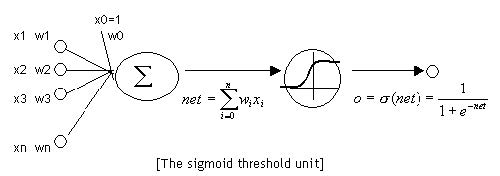
\includegraphics[width=0.7\textwidth]{Bp1.jpg}
	\caption{神经元}
	\label{fig:Bp1}
\end{figure}

计算一个神经元的输出的方法和计算一个感知器的输出是一样的。假设神经元的输入是向量\(\vec{x}\),权重向量是\(\vec{w}\)(偏置项是\(w_0\)),激活函数是sigmoid函数,则其输出\(y\):

\begin{equation}
	\label{eq:Bp1}
	y=sigmoid(\vec{w}^T\centerdot\vec{x})
\end{equation}


sigmoid函数的定义如下:
\[
	sigmoid(x)=\frac{1}{1+e^{-x}}
\]
将其带入前面的式子,得到
\[
	y=\frac{1}{1+e^{-\vec{w}^T\centerdot\vec{x}}}
\]
sigmoid函数是一个非线性函数,值域是(0,1)。函数图像如图\ref{fig:Bp2}所示

\begin{figure}[htbp]
	\centering
	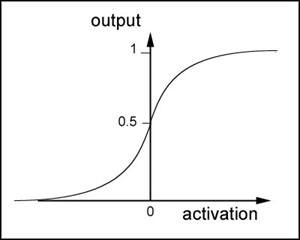
\includegraphics[width=0.5\textwidth]{Bp2.jpg}
	\caption{sigmoid函数}
	\label{fig:Bp2}
\end{figure}

sigmoid函数的导数是:
\begin{align*}
	 & \mbox{令} y=sigmoid(x) \\
	 & \mbox{则} y'=y(1-y)
\end{align*}


可以看到,sigmoid函数的导数非常有趣,它可以用sigmoid函数自身来表示。这样,一旦计算出sigmoid函数的值,计算它的导数的值就非常方便。


\section{神经网络是啥}\label{Bp:2}

\begin{figure}[htbp]
	\centering
	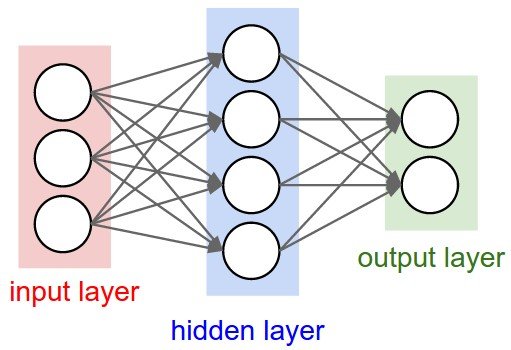
\includegraphics[width=0.5\textwidth]{Bp3.jpeg}
	\caption{Bp神经网络}
	\label{fig:Bp3}
\end{figure}

神经网络其实就是按照\textbf{一定规则}连接起来的多个\textbf{神经元}。图\ref{fig:Bp3}展示了一个\textbf{全连接(full connected, FC)}神经网络,通过观察可以发现它的规则包括:

\begin{itemize}
	\item
	      神经元按照\textbf{层}来布局。最左边的层叫做\textbf{输入层},负责接收输入数据;最右边的层叫\textbf{输出层},我们可以从这层获取神经网络输出数据。输入层和输出层之间的层叫做\textbf{隐藏层},因为它们对于外部来说是不可见的。
	\item
	      同一层的神经元之间没有连接。
	\item
	      第N层的每个神经元和第N-1层的\textbf{所有}神经元相连(这就是full connected的含义),第N-1层神经元的输出就是第N层神经元的输入。
	\item
	      每个连接都有一个\textbf{权值}。
\end{itemize}

上面这些规则定义了全连接神经网络的结构。事实上还存在很多其它结构的神经网络,比如卷积神经网络(CNN)、循环神经网络(RNN),他们都具有不同的连接规则。


\section{计算神经网络的输出}\label{Bp:3}

神经网络实际上就是一个输入向量\(\vec{x}\)到输出向量\(\vec{y}\)的函数,即:
\[
	\vec{y} = f_{network}(\vec{x})
\]

根据输入计算神经网络的输出,需要首先将输入向量\(\vec{x}\)的每个元素{}\(x_i\)的值赋给神经网络的输入层的对应神经元,然后根据公式\ref{eq:Bp1}依次向前计算每一层的每个神经元的值,直到最后一层输出层的所有神经元的值计算完毕。最后,将输出层每个神经元的值串在一起就得到了输出向量\(\vec{y}\)。

接下来举一个例子来说明这个过程,我们先给神经网络的每个单元写上编号。

\begin{figure}[htbp]
	\centering
	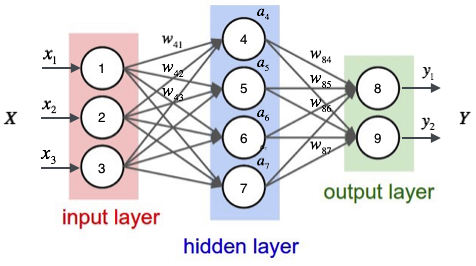
\includegraphics[width=0.7\textwidth]{Bp4.png}
	\caption{神经网络}
	\label{fig:Bp4}
\end{figure}

如上图,输入层有三个节点,我们将其依次编号为1、2、3;隐藏层的4个节点,编号依次为4、5、6、7;最后输出层的两个节点编号为8、9。因为我们这个神经网络是\textbf{全连接}网络,所以可以看到每个节点都和\textbf{上一层的所有节点}有连接。比如,我们可以看到隐藏层的节点4,它和输入层的三个节点1、2、3之间都有连接,其连接上的权重分别为\(w_{41},w_{42},w_{43}\)。那么,我们怎样计算节点4的输出值\(a_4\)呢?

为了计算节点4的输出值,我们必须先得到其所有上游节点(也就是节点1、2、3)的输出值。节点1、2、3是\textbf{输入层}的节点,所以,他们的输出值就是输入向量\(\vec{x}\)本身。按照上图画出的对应关系,可以看到节点1、2、3的输出值分别是\(x_1,x_2,x_3\)。我们要求\textbf{输入向量的维度和输入层神经元个数相同},而输入向量的某个元素对应到哪个输入节点是可以自由决定的,你偏非要把\(x_1\)赋值给节点2也是完全没有问题的,但这样除了把自己弄晕之外,并没有什么价值。

一旦我们有了节点1、2、3的输出值,我们就可以根据公式\ref{eq:Bp1}计算节点4的输出值\(a_4\):
\begin{align*}
	a_4 & =sigmoid(\vec{w}^T\centerdot\vec{x})           \\
	    & =sigmoid(w_{41}x_1+w_{42}x_2+w_{43}x_3+w_{4b})
\end{align*}


上式的\(w_{4b}\)是节点4的\textbf{偏置项},图中没有画出来。而\(w_{41},w_{42},w_{43}\)分别为节点1、2、3到节点4连接的权重,在给权重\(w_{ji}\)编号时,我们把目标节点的编号\(j\)放在前面,把源节点的编号\(i\)放在后面。

同样,我们可以继续计算出节点5、6、7的输出值\(a_5,a_6,a_7\)。这样,隐藏层的4个节点的输出值就计算完成了,我们就可以接着计算输出层的节点8的输出值\(y_1\):
\begin{align*}
	y_1 & =sigmoid(\vec{w}^T\centerdot\vec{a})                     \\
	    & =sigmoid(w_{84}a_4+w_{85}a_5+w_{86}a_6+w_{87}a_7+w_{8b})
\end{align*}

同理,我们还可以计算出\(y_2\)的值。这样输出层所有节点的输出值计算完毕,我们就得到了在输入向量\(\vec{x}=\begin{bmatrix}x_1\\x_2\\x_3\end{bmatrix}\)时,神经网络的输出向量\(\vec{y}=\begin{bmatrix}y_1\\y_2\end{bmatrix}\)。这里我们也看到,\textbf{输出向量的维度和输出层神经元个数相同}。


\section{神经网络的矩阵表示}\label{Bp:4}

神经网络的计算如果用矩阵来表示会很方便(当然逼格也更高),我们先来看看隐藏层的矩阵表示。

首先我们把隐藏层4个节点的计算依次排列出来:
\begin{align*}
	a_4 & =sigmoid(w_{41}x_1+w_{42}x_2+w_{43}x_3+w_{4b}) \\
	a_5 & =sigmoid(w_{51}x_1+w_{52}x_2+w_{53}x_3+w_{5b}) \\
	a_6 & =sigmoid(w_{61}x_1+w_{62}x_2+w_{63}x_3+w_{6b}) \\
	a_7 & =sigmoid(w_{71}x_1+w_{72}x_2+w_{73}x_3+w_{7b})
\end{align*}

接着,定义网络的输入向量\(\vec{x}\)和隐藏层每个节点的权重向量\(\vec{w_j}\)。令
\[\vec{x}=\begin{bmatrix}x_1\\x_2\\x_3\\1\end{bmatrix}\]
\begin{align*}
	\vec{w}_4 & =[w_{41},w_{42},w_{43},w_{4b}] \\
	\vec{w}_5 & =[w_{51},w_{52},w_{53},w_{5b}] \\
	\vec{w}_6 & =[w_{61},w_{62},w_{63},w_{6b}] \\
	\vec{w}_7 & =[w_{71},w_{72},w_{73},w_{7b}] \\
	f         & =sigmoid
\end{align*}


代入到前面的一组式子,得到:
\begin{align*}
	a_4 & =f(\vec{w_4}\centerdot\vec{x}),\qquad
	a_5=f(\vec{w_5}\centerdot\vec{x})           \\
	a_6 & =f(\vec{w_6}\centerdot\vec{x}),\qquad
	a_7=f(\vec{w_7}\centerdot\vec{x})
\end{align*}


现在,我们把上述计算\(a_4,a_5,a_6,a_7\)的四个式子写到一个矩阵里面,每个式子作为矩阵的一行,就可以利用矩阵来表示它们的计算了。令
\[
	\vec{a}=
	\begin{bmatrix}
		a_4 \\
		a_5 \\
		a_6 \\
		a_7 \\
	\end{bmatrix},\qquad W=
	\begin{bmatrix}
		\vec{w}_4 \\
		\vec{w}_5 \\
		\vec{w}_6 \\
		\vec{w}_7 \\
	\end{bmatrix}=
	\begin{bmatrix}
		w_{41},w_{42},w_{43},w_{4b} \\
		w_{51},w_{52},w_{53},w_{5b} \\
		w_{61},w_{62},w_{63},w_{6b} \\
		w_{71},w_{72},w_{73},w_{7b} \\
	\end{bmatrix}
	,\qquad f(
	\begin{bmatrix}
		x_1 \\
		x_2 \\
		x_3 \\
		.   \\
		.   \\
		.   \\
	\end{bmatrix})=
	\begin{bmatrix}
		f(x_1) \\
		f(x_2) \\
		f(x_3) \\
		.      \\
		.      \\
		.      \\
	\end{bmatrix}
\]

带入前面的一组式子,得到
\begin{equation}
	\label{eq:Bp2}
	\vec{a}=f(W\centerdot\vec{x})
\end{equation}

在公式\ref{eq:Bp2}中,\(f\)是激活函数,在本例中是\(sigmoid\)函数;\(W\)是某一层的权重矩阵;\(\vec{x}\)是某层的输入向量;\(\vec{a}\)是某层的输出向量。公式\ref{eq:Bp2}说明神经网络的每一层的作用实际上就是先将输入向量\textbf{左乘}一个数组进行线性变换,得到一个新的向量,然后再对这个向量\textbf{逐元素}应用一个激活函数。

每一层的算法都是一样的。比如,对于包含一个输入层,一个输出层和三个隐藏层的神经网络,我们假设其权重矩阵分别为\(W_1,W_2,W_3,W_4\),每个隐藏层的输出分别是\(\vec{a}_1,\vec{a}_2,\vec{a}_3\),神经网络的输入为\(\vec{x}\),神经网络的输入为\(\vec{y}\),如图\ref{fig:Bp5}所示:

\begin{figure}[htbp]
	\centering
	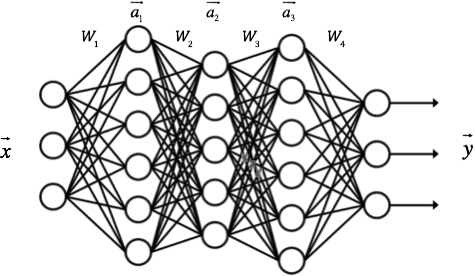
\includegraphics[width=0.7\textwidth]{Bp5.png}
	\caption{神经网络}
	\label{fig:Bp5}
\end{figure}

则每一层的输出向量的计算可以表示为:
\begin{align*}
	 & \vec{a}_1=f(W_1\centerdot\vec{x}),\qquad \vec{a}_2=f(W_2\centerdot\vec{a}_1) \\
	 & \vec{a}_3=f(W_3\centerdot\vec{a}_2),\qquad\vec{y}=f(W_4\centerdot\vec{a}_3)
\end{align*}


这就是神经网络输出值的计算方法。


\section{神经网络的训练}\label{Bp:5}

现在,我们需要知道一个神经网络的每个连接上的权值是如何得到的。我们可以说神经网络是一个\textbf{模型},那么这些权值就是模型的\textbf{参数},也就是模型要学习的东西。然而,一个神经网络的连接方式、网络的层数、每层的节点数这些参数,则不是学习出来的,而是人为事先设置的。对于这些人为设置的参数,我们称之为\textbf{超参数(Hyper-Parameters)}。

接下来,我们将要介绍神经网络的训练算法:反向传播算法。


\subsection{反向传播算法(Back Propagation)}\label{Bp:6}

我们首先直观的介绍反向传播算法,最后再来介绍这个算法的推导。当然读者也可以完全跳过推导部分,因为即使不知道如何推导,也不影响你写出来一个神经网络的训练代码。事实上,现在神经网络成熟的开源实现多如牛毛,除了练手之外,你可能都没有机会需要去写一个神经网络。

我们以\textbf{监督学习}为例来解释反向传播算法。在第\ref{chap:Line}章中我们介绍了什么是\textbf{监督学习},如果忘记了可以再看一下。另外,我们设神经元的激活函数\(f\)为\(sigmoid\)函数(不同激活函数的计算公式不同,详情见\ref{Bp:7}反向传播算法的推导一节)。

我们假设每个训练样本为\((\vec{x},\vec{t})\),其中向量\(\vec{x}\)是训练样本的特征,而\(\vec{t}\)是样本的目标值。

首先,我们根据上一节介绍的算法,用样本的特征\(\vec{x}\),计算出神经网络中每个隐藏层节点的输出\(a_i\),以及输出层每个节点的输出\(y_i\)。

然后,我们按照下面的方法计算出每个节点的误差项\(\delta_i\):

\begin{itemize}
	\item
	      对于输出层节点\(i\),
	      \begin{equation}
		      \label{eq:Bp3}
		      \delta_i=y_i(1-y_i)(t_i-y_i)
	      \end{equation}

\end{itemize}
其中,\(\delta_i\)是节点\(i\)的误差项,\(y_i\)是节点\(i\)的\textbf{输出值},\(t_i\)是样本对应于节点\(i\)的\textbf{目标值}。举个例子,根据上图,对于输出层节点8来说,它的输出值是\(y_1\),而样本的目标值是\(t_1\),带入上面的公式得到节点8的误差项\(\delta_8\)应该是:
\[
	\delta_8=y_1(1-y_1)(t_1-y_1)
\]

\begin{itemize}
	\item
	      对于隐藏层节点,
	      \begin{equation}
		      \label{eq:Bp4}
		      \delta_i=a_i(1-a_i)\sum_{k\in{outputs}}w_{ki}\delta_k
	      \end{equation}
\end{itemize}
其中,\(a_i\)是节点\(i\)的输出值,\(w_{ki}\)是节点\(i\)到它的下一层节点\(k\)的连接的权重,\(\delta_k\)是节点\(i\)的下一层节点\(k\)的误差项。例如,对于隐藏层节点4来说,计算方法如下:
\[
	\delta_4=a_4(1-a_4)(w_{84}\delta_8+w_{94}\delta_9)
\]
最后,更新每个连接上的权值:
\begin{equation}
	\label{eq:Bp5}
	w_{ji}\gets w_{ji}+\eta\delta_jx_{ji}
\end{equation}
其中,\(w_{ji}\)是节点\(i\)到节点\(j\)的权重,\(\eta\)是一个成为\textbf{学习速率}的常数,\(\delta_j\)是节点的误差项,\(x_{ji}\)是节点\(i\)传递给节点\(j\)的输入。例如,权重\(w_84\)的更新方法如下:
\[
	w_{84}\gets w_{84}+\eta\delta_8 a_4
\]
类似的,权重\(w_{41}\)的更新方法如下:
\[
	w_{41}\gets w_{41}+\eta\delta_4 x_1
\]

偏置项的输入值永远为1。例如,节点4的偏置项\(w_{4b}\)应该按照下面的方法计算:
\[
	w_{4b}\gets w_{4b}+\eta\delta_4
\]

我们已经介绍了神经网络每个节点误差项的计算和权重更新方法。显然,计算一个节点的误差项,需要先计算每个与其相连的下一层节点的误差项。这就要求误差项的计算顺序必须是从输出层开始,然后反向依次计算每个隐藏层的误差项,直到与输入层相连的那个隐藏层。这就是反向传播算法的名字的含义。当所有节点的误差项计算完毕后,我们就可以根据公式\ref{eq:Bp5}来更新所有的权重。

以上就是基本的反向传播算法,并不是很复杂,您弄清楚了么?




\subsection{反向传播算法的推导}\label{Bp:7}
反向传播算法其实就是链式求导法则的应用。然而,这个如此简单且显而易见的方法,却是在Roseblatt提出感知器算法将近30年之后才被发明和普及的。对此,Bengio这样回应道:

\begin{note}
	很多看似显而易见的想法只有在事后才变得显而易见。
\end{note}

接下来,我们用链式求导法则来推导反向传播算法,也就是上一小节的公式\ref{eq:Bp3}, \ref{eq:Bp4}, \ref{eq:Bp5}。

% \textbf{\emph{前方高能预警——接下来是数学公式重灾区,读者可以酌情阅读,不必强求。}}

按照机器学习的通用套路,我们先确定神经网络的目标函数,然后用\textbf{随机梯度下降}优化算法去求目标函数最小值时的参数值。

我们取网络所有输出层节点的误差平方和作为目标函数:
\[
	E_d\equiv\frac{1}{2}\sum_{i\in outputs}(t_i-y_i)^2
\]

其中,\(E_d\)表示是样本\(d\)的误差。

然后,我们用第\ref{chap:Line}章中介绍的\textbf{随机梯度下降}算法对目标函数进行优化:
\[
	w_{ji}\gets w_{ji}-\eta\frac{\partial{E_d}}{\partial{w_{ji}}}
\]

随机梯度下降算法也就是需要求出误差\(E_d\)对于每个权重\(w_{ji}\)的偏导数(也就是梯度),怎么求呢?观察图\ref{fig:Bp4},我们发现权重\(w_{ji}\)仅能通过影响节点\(j\)的输入值影响网络的其它部分,设\(net_j\)是节点\(j\)的\textbf{加权输入},即
\begin{align*}
	net_j=\vec{w_j}\centerdot\vec{x_j} =\sum_{i}{w_{ji}}x_{ji}
\end{align*}
\(E_d\)是\(net_j\)的函数,而\(net_j\)是\(w_{ji}\)的函数。根据链式求导法则,可以得到:
\begin{align*}
	\frac{\partial{E_d}}{\partial{w_{ji}}}=\frac{\partial{E_d}}{\partial{net_j}}\frac{\partial{net_j}}{\partial{w_{ji}}}=\frac{\partial{E_d}}{\partial{net_j}}\frac{\partial{\sum_{i}{w_{ji}}x_{ji}}}{\partial{w_{ji}}}=\frac{\partial{E_d}}{\partial{net_j}}x_{ji}
\end{align*}
上式中,\(x_{ji}\)是节点\(i\)传递给节点\(j\)的输入值,也就是节点\(i\)的输出值。

对于\(\frac{\partial{E_d}}{\partial{net_j}}\)的推导,需要区分\textbf{输出层}和\textbf{隐藏层}两种情况。


\textbf{输出层权值训练}

对于\textbf{输出层}来说,\(net_j\)仅能通过节点\(j\)的输出值\(y_j\)来影响网络其它部分,也就是说\(E_d\)是\(y_j\)的函数,而\(y_j\)是\(net_j\)的函数,其中\(y_j=sigmoid(net_j)\)。所以我们可以再次使用链式求导法则:
\begin{align*}
	\frac{\partial{E_d}}{\partial{net_j}} & =\frac{\partial{E_d}}{\partial{y_j}}\frac{\partial{y_j}}{\partial{net_j}}
\end{align*}


考虑上式第一项:
\begin{align*}
	\frac{\partial{E_d}}{\partial{y_j}} & =\frac{\partial}{\partial{y_j}}\frac{1}{2}\sum_{i\in outputs}(t_i-y_i)^2 \\
	                                    & =\frac{\partial}{\partial{y_j}}\frac{1}{2}(t_j-y_j)^2                    \\
	                                    & =-(t_j-y_j)
\end{align*}


考虑上式第二项:
\begin{align*}
	\frac{\partial{y_j}}{\partial{net_j}} & =\frac{\partial sigmoid(net_j)}{\partial{net_j}} \\
	                                      & =y_j(1-y_j)
\end{align*}


将第一项和第二项带入,得到:
\[
	\frac{\partial{E_d}}{\partial{net_j}}=-(t_j-y_j)y_j(1-y_j)
\]

如果令\(\delta_j=-\frac{\partial{E_d}}{\partial{net_j}}\),也就是一个节点的误差项\(\delta\)是网络误差对这个节点输入的偏导数的相反数。带入上式,得到:
\[
	\delta_j=(t_j-y_j)y_j(1-y_j)
\]

上式就是公式\ref{eq:Bp3}。

将上述推导带入随机梯度下降公式,得到:
\begin{align*}
	w_{ji} & \gets w_{ji}-\eta\frac{\partial{E_d}}{\partial{w_{ji}}} \\
	       & =w_{ji}+\eta(t_j-y_j)y_j(1-y_j)x_{ji}                   \\
	       & =w_{ji}+\eta\delta_jx_{ji}
\end{align*}


上式就是公式\ref{eq:Bp5}。

\textbf{隐藏层权值训练}

现在我们要推导出隐藏层的\(\frac{\partial{E_d}}{\partial{net_j}}\)。

首先,我们需要定义节点\(j\)的所有直接下游节点的集合\(Downstream(j)\)。例如,对于节点4来说,它的直接下游节点是节点8、节点9。可以看到\(net_j\)只能通过影响\(Downstream(j)\)再影响\(E_d\)。设\(net_k\)是节点\(j\)的下游节点的输入,则\(E_d\)是\(net_k\)的函数,而\(net_k\)是\(net_j\)的函数。因为\(net_k\)有多个,我们应用全导数公式,可以做出如下推导:
\begin{align*}
	\frac{\partial{E_d}}{\partial{net_j}} & =\sum_{k\in Downstream(j)}\frac{\partial{E_d}}{\partial{net_k}}\frac{\partial{net_k}}{\partial{net_j}}        \\
	                                      & =\sum_{k\in Downstream(j)}-\delta_k\frac{\partial{net_k}}{\partial{net_j}}                                    \\
	                                      & =\sum_{k\in Downstream(j)}-\delta_k\frac{\partial{net_k}}{\partial{a_j}}\frac{\partial{a_j}}{\partial{net_j}} \\
	                                      & =\sum_{k\in Downstream(j)}-\delta_kw_{kj}\frac{\partial{a_j}}{\partial{net_j}}                                \\
	                                      & =\sum_{k\in Downstream(j)}-\delta_kw_{kj}a_j(1-a_j)                                                           \\
	                                      & =-a_j(1-a_j)\sum_{k\in Downstream(j)}\delta_kw_{kj}
\end{align*}

因为\(\delta_j=-\frac{\partial{E_d}}{\partial{net_j}}\),带入上式得到:
\[
	\delta_j=a_j(1-a_j)\sum_{k\in Downstream(j)}\delta_kw_{kj}
\]

上式就是公式\ref{eq:Bp4}。

\textbf{——数学公式警报解除——}

至此,我们已经推导出了反向传播算法。需要注意的是,我们刚刚推导出的训练规则是根据激活函数是sigmoid函数、平方和误差、全连接网络、随机梯度下降优化算法。如果激活函数不同、误差计算方式不同、网络连接结构不同、优化算法不同,则具体的训练规则也会不一样。但是无论怎样,训练规则的推导方式都是一样的,应用链式求导法则进行推导即可。


\section{编程实战:神经网络的实现}\label{Bp:8}
\begin{note}
	完整代码请参考GitHub:\url{https://github.com/hanbt/learn_dl/blob/master/bp.py} (python2.7)
\end{note}

现在,我们要根据前面的算法,实现一个基本的全连接神经网络,这并不需要太多代码。我们在这里依然采用面向对象设计。

首先,我们先做一个基本的模型:

\begin{figure}[htbp]
	\centering
	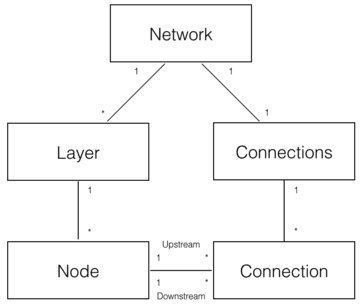
\includegraphics[width=0.4\textwidth]{Bp6.png}
	\caption{基础模型}
	\label{fig:Bp6}
\end{figure}
如图\ref{fig:Bp6},可以分解出5个领域对象来实现神经网络:
\begin{itemize}
	\item
	      \emph{Network}
	      神经网络对象,提供API接口。它由若干层对象组成以及连接对象组成。
	\item
	      \emph{Layer} 层对象,由多个节点组成。
	\item
	      \emph{Node} 节点对象计算和记录节点自身的信息(比如输出值\(a\)、误差项\(\delta\)等),以及与这个节点相关的上下游的连接。
	\item
	      \emph{Connection} 每个连接对象都要记录该连接的权重。
	\item
	      \emph{Connections} 仅仅作为Connection的集合对象,提供一些集合操作。
\end{itemize}

Node实现如下:
\begin{lstlisting}
# 节点类,负责记录和维护节点自身信息以及与这个节点相关的上下游连接,实现输出值和误差项的计算。
class Node(object):
    def __init__(self, layer_index, node_index):
        '''
        构造节点对象。
        layer_index: 节点所属的层的编号
        node_index: 节点的编号
        '''
        self.layer_index = layer_index
        self.node_index = node_index
        self.downstream = []
        self.upstream = []
        self.output = 0
        self.delta = 0
    def set_output(self, output):
        '''
        设置节点的输出值。如果节点属于输入层会用到这个函数。
        '''
        self.output = output
    def append_downstream_connection(self, conn):
        '''
        添加一个到下游节点的连接
        '''
        self.downstream.append(conn)
    def append_upstream_connection(self, conn):
        '''
        添加一个到上游节点的连接
        '''
        self.upstream.append(conn)
    def calc_output(self):
        '''
        根据式1计算节点的输出
        '''
        output = reduce(lambda ret, conn: ret + conn.upstream_node.output * conn.weight, self.upstream, 0)
        self.output = sigmoid(output)
    def calc_hidden_layer_delta(self):
        '''
        节点属于隐藏层时,根据式4计算delta
        '''
        downstream_delta = reduce(
            lambda ret, conn: ret + conn.downstream_node.delta * conn.weight,
            self.downstream, 0.0)
        self.delta = self.output * (1 - self.output) * downstream_delta
    def calc_output_layer_delta(self, label):
        '''
        节点属于输出层时,根据式3计算delta
        '''
        self.delta = self.output * (1 - self.output) * (label - self.output)
    def __str__(self):
        '''
        打印节点的信息
        '''
        node_str = '%u-%u: output: %f delta: %f' % (self.layer_index, self.node_index, self.output, self.delta)
        downstream_str = reduce(lambda ret, conn: ret + '\n\t' + str(conn), self.downstream, '')
        upstream_str = reduce(lambda ret, conn: ret + '\n\t' + str(conn), self.upstream, '')
        return node_str + '\n\tdownstream:' + downstream_str + '\n\tupstream:' + upstream_str 
\end{lstlisting}

ConstNode对象,为了实现一个输出恒为1的节点(计算偏置项\(w_b\)时需要)
\begin{lstlisting}
class ConstNode(object):
    def __init__(self, layer_index, node_index):
        '''
        构造节点对象。
        layer_index: 节点所属的层的编号
        node_index: 节点的编号
        '''    
        self.layer_index = layer_index
        self.node_index = node_index
        self.downstream = []
        self.output = 1
    def append_downstream_connection(self, conn):
        '''
        添加一个到下游节点的连接
        '''       
        self.downstream.append(conn)
    def calc_hidden_layer_delta(self):
        '''
        节点属于隐藏层时,根据式4计算delta
        '''
        downstream_delta = reduce(
            lambda ret, conn: ret + conn.downstream_node.delta * conn.weight,
            self.downstream, 0.0)
        self.delta = self.output * (1 - self.output) * downstream_delta
    def __str__(self):
        '''
        打印节点的信息
        '''
        node_str = '%u-%u: output: 1' % (self.layer_index, self.node_index)
        downstream_str = reduce(lambda ret, conn: ret + '\n\t' + str(conn), self.downstream, '')
        return node_str + '\n\tdownstream:' + downstream_str
\end{lstlisting}


Layer对象,负责初始化一层。此外,作为Node的集合对象,提供对Node集合的操作。
\begin{lstlisting}
class Layer(object):
    def __init__(self, layer_index, node_count):
        '''
        初始化一层
        layer_index: 层编号
        node_count: 层所包含的节点个数
        '''
        self.layer_index = layer_index
        self.nodes = []
        for i in range(node_count):
            self.nodes.append(Node(layer_index, i))
        self.nodes.append(ConstNode(layer_index, node_count))
    def set_output(self, data):
        '''
        设置层的输出。当层是输入层时会用到。
        '''
        for i in range(len(data)):
            self.nodes[i].set_output(data[i])
    def calc_output(self):
        '''
        计算层的输出向量
        '''
        for node in self.nodes[:-1]:
            node.calc_output()
    def dump(self):
        '''
        打印层的信息
        '''
        for node in self.nodes:
            print node
\end{lstlisting}

Connection对象,主要职责是记录连接的权重,以及这个连接所关联的上下游节点。
\begin{lstlisting}
class Connection(object):
    def __init__(self, upstream_node, downstream_node):
        '''
        初始化连接,权重初始化为是一个很小的随机数
        upstream_node: 连接的上游节点
        downstream_node: 连接的下游节点
        '''
        self.upstream_node = upstream_node
        self.downstream_node = downstream_node
        self.weight = random.uniform(-0.1, 0.1)
        self.gradient = 0.0
    def calc_gradient(self):
        '''
        计算梯度
        '''
        self.gradient = self.downstream_node.delta * self.upstream_node.output
    def get_gradient(self):
        '''
        获取当前的梯度
        '''
        return self.gradient
    def update_weight(self, rate):
        '''
        根据梯度下降算法更新权重
        '''
        self.calc_gradient()
        self.weight += rate * self.gradient
    def __str__(self):
        '''
        打印连接信息
        '''
        return '(%u-%u) -> (%u-%u) = %f' % (
            self.upstream_node.layer_index, 
            self.upstream_node.node_index,
            self.downstream_node.layer_index, 
            self.downstream_node.node_index, 
            self.weight)
\end{lstlisting}

Connections对象,提供Connection集合操作。
\begin{lstlisting}
class Connections(object):
    def __init__(self):
        self.connections = []
    def add_connection(self, connection):
        self.connections.append(connection)
    def dump(self):
        for conn in self.connections:
            print conn
\end{lstlisting}

Network对象,提供API。
\begin{lstlisting}
class Network(object):
    def __init__(self, layers):
        '''
        初始化一个全连接神经网络
        layers: 二维数组,描述神经网络每层节点数
        '''
        self.connections = Connections()
        self.layers = []
        layer_count = len(layers)
        node_count = 0;
        for i in range(layer_count):
            self.layers.append(Layer(i, layers[i]))
        for layer in range(layer_count - 1):
            connections = [Connection(upstream_node, downstream_node) 
                           for upstream_node in self.layers[layer].nodes
                           for downstream_node in self.layers[layer + 1].nodes[:-1]]
            for conn in connections:
                self.connections.add_connection(conn)
                conn.downstream_node.append_upstream_connection(conn)
                conn.upstream_node.append_downstream_connection(conn)
    def train(self, labels, data_set, rate, iteration):
        '''
        训练神经网络
        labels: 数组,训练样本标签。每个元素是一个样本的标签。
        data_set: 二维数组,训练样本特征。每个元素是一个样本的特征。
        '''
        for i in range(iteration):
            for d in range(len(data_set)):
                self.train_one_sample(labels[d], data_set[d], rate)
    def train_one_sample(self, label, sample, rate):
        '''
        内部函数,用一个样本训练网络
        '''
        self.predict(sample)
        self.calc_delta(label)
        self.update_weight(rate)
    def calc_delta(self, label):
        '''
        内部函数,计算每个节点的delta
        '''
        output_nodes = self.layers[-1].nodes
        for i in range(len(label)):
            output_nodes[i].calc_output_layer_delta(label[i])
        for layer in self.layers[-2::-1]:
            for node in layer.nodes:
                node.calc_hidden_layer_delta()
    def update_weight(self, rate):
        '''
        内部函数,更新每个连接权重
        '''
        for layer in self.layers[:-1]:
            for node in layer.nodes:
                for conn in node.downstream:
                    conn.update_weight(rate)
    def calc_gradient(self):
        '''
        内部函数,计算每个连接的梯度
        '''
        for layer in self.layers[:-1]:
            for node in layer.nodes:
                for conn in node.downstream:
                    conn.calc_gradient()
    def get_gradient(self, label, sample):
        '''
        获得网络在一个样本下,每个连接上的梯度
        label: 样本标签
        sample: 样本输入
        '''
        self.predict(sample)
        self.calc_delta(label)
        self.calc_gradient()
    def predict(self, sample):
        '''
        根据输入的样本预测输出值
        sample: 数组,样本的特征,也就是网络的输入向量
        '''
        self.layers[0].set_output(sample)
        for i in range(1, len(self.layers)):
            self.layers[i].calc_output()
        return map(lambda node: node.output, self.layers[-1].nodes[:-1])
    def dump(self):
        '''
        打印网络信息
        '''
        for layer in self.layers:
            layer.dump()
\end{lstlisting}

至此,实现了一个基本的全连接神经网络。可以看到,同神经网络的强大学习能力相比,其实现还算是很容易的。

\textbf{梯度检查}

怎么保证自己写的神经网络没有BUG呢?事实上这是一个非常重要的问题。一方面,千辛万苦想到一个算法,结果效果不理想,那么是算法本身错了还是代码实现错了呢?定位这种问题肯定要花费大量的时间和精力。另一方面,由于神经网络的复杂性,我们几乎无法事先知道神经网络的输入和输出,因此类似TDD(测试驱动开发)这样的开发方法似乎也不可行。

办法还是有滴,就是利用梯度检查来确认程序是否正确。梯度检查的思路如下:

对于梯度下降算法:
\[
	w_{ji}\gets w_{ji}-\eta\frac{\partial{E_d}}{\partial{w_{ji}}}
\]

来说,这里关键之处在于\(\frac{\partial{E_d}}{\partial{w_{ji}}}\)的计算一定要正确,而它是\(E_d\)对\(w_{ji}\)的\emph{偏导数}。而根据导数的定义:
\[
	f'(\theta)=\lim_{\epsilon->0}\frac{f(\theta+\epsilon)-f(\theta-\epsilon)}{2\epsilon}
\]

对于任意\(\theta\)的导数值,我们都可以用等式右边来近似计算。我们把\(E_d\)看做是\(w_{ji}\)的函数,即\(E_d(w_{ji})\),那么根据导数定义,\(\frac{\partial{E_d(w_{ji})}}{\partial{w_{ji}}}\)应该等于:
\[
	\frac{\partial{E_d(w_{ji})}}{\partial{w_{ji}}}=\lim_{\epsilon->0}\frac{f(w_{ji}+\epsilon)-f(w_{ji}-\epsilon)}{2\epsilon}
\]

如果把\(\epsilon\)设置为一个很小的数(比如\(10^{-4}\)),那么上式可以写成:
\begin{equation}
	\label{eq:Bp6}
	\frac{\partial{E_d(w_{ji})}}{\partial{w_{ji}}}\approx\frac{f(w_{ji}+\epsilon)-f(w_{ji}-\epsilon)}{2\epsilon}
\end{equation}


我们就可以利用公式\ref{eq:Bp6},来计算梯度\(\frac{\partial{E_d}}{\partial{w_{ji}}}\)的值,然后同我们神经网络代码中计算出来的梯度值进行比较。如果两者的差别\textbf{非常的小},那么就说明我们的代码是正确的。

下面是梯度检查的代码。如果我们想检查参数\(w_{ji}\)的梯度是否正确,我们需要以下几个步骤:

\begin{enumerate}
	\item
	      首先使用一个样本\(d\)对神经网络进行训练,这样就能获得每个权重的梯度。
	\item
	      将\(w_{ji}\)加上一个很小的值(\(10^{-4}\)),重新计算神经网络在这个样本\(d\)下的\(E_{d+}\)。
	\item
	      将\(w_{ji}\)减上一个很小的值(\(10^{-4}\)),重新计算神经网络在这个样本\(d\)下的\(E_{d-}\)。
	\item
	      根据公式\ref{eq:Bp6}计算出期望的梯度值,和第一步获得的梯度值进行比较,它们应该几乎想等(至少4位有效数字相同)。
\end{enumerate}

当然,我们可以重复上面的过程,对每个权重\(w_{ji}\)都进行检查。也可以使用多个样本重复检查。
\begin{lstlisting}
def gradient_check(network, sample_feature, sample_label):
    '''
    梯度检查
    network: 神经网络对象
    sample_feature: 样本的特征
    sample_label: 样本的标签
    '''
    # 计算网络误差
    network_error = lambda vec1, vec2: \
            0.5 * reduce(lambda a, b: a + b, 
                      map(lambda v: (v[0] - v[1]) * (v[0] - v[1]),
                          zip(vec1, vec2)))
    # 获取网络在当前样本下每个连接的梯度
    network.get_gradient(sample_feature, sample_label)
    # 对每个权重做梯度检查    
    for conn in network.connections.connections: 
        # 获取指定连接的梯度
        actual_gradient = conn.get_gradient()
        # 增加一个很小的值,计算网络的误差
        epsilon = 0.0001
        conn.weight += epsilon
        error1 = network_error(network.predict(sample_feature), sample_label)
        # 减去一个很小的值,计算网络的误差
        conn.weight -= 2 * epsilon # 刚才加过了一次,因此这里需要减去2倍
        error2 = network_error(network.predict(sample_feature), sample_label)
        # 根据式6计算期望的梯度值
        expected_gradient = (error2 - error1) / (2 * epsilon)
        # 打印
        print 'expected gradient: \t%f\nactual gradient: \t%f' % (
            expected_gradient, actual_gradient)
\end{lstlisting}

至此,会推导、会实现、会抓BUG,你已经摸到深度学习的大门了。接下来还需要不断的实践,我们用刚刚写过的神经网络去识别手写数字。


\section{神经网络实战:手写数字识别}\label{Bp:9}
针对这个任务,我们采用业界非常流行的MNIST数据集。MNIST大约有60000个手写字母的训练样本,我们使用它训练我们的神经网络,然后再用训练好的网络去识别手写数字。

手写数字识别是个比较简单的任务,数字只可能是0-9中的一个,这是个10分类问题。

\subsection{超参数的确定}\label{Bp:10}

我们首先需要确定网络的层数和每层的节点数。关于第一个问题,实际上并没有什么理论化的方法,大家都是根据经验来拍,如果没有经验的话就随便拍一个。然后,你可以多试几个值,训练不同层数的神经网络,看看哪个效果最好就用哪个。嗯,现在你可能明白为什么说深度学习是个手艺活了,有些手艺很让人无语,而有些手艺还是很有技术含量的。

不过,有些基本道理我们还是明白的,我们知道网络层数越多越好,也知道层数越多训练难度越大。对于全连接网络,隐藏层最好不要超过三层。那么,我们可以先试试仅有一个隐藏层的神经网络效果怎么样。毕竟模型小的话,训练起来也快些(刚开始玩模型的时候,都希望快点看到结果)。

输入层节点数是确定的。因为MNIST数据集每个训练数据是28*28的图片,共784个像素,因此,输入层节点数应该是784,每个像素对应一个输入节点。

输出层节点数也是确定的。因为是10分类,我们可以用10个节点,每个节点对应一个分类。输出层10个节点中,输出最大值的那个节点对应的分类,就是模型的预测结果。

隐藏层节点数量是不好确定的,从1到100万都可以。下面有几个经验公式:
\begin{align*}
	 & m=\sqrt{n+l}+\alpha \\
	 & m=log_2n            \\
	 & m=\sqrt{nl}
\end{align*}
其中,$m$:隐藏层节点数;$n$:输入层节点数;$l$:输出层节点数;$\alpha$:1到10之间的常数。
因此,我们可以先根据上面的公式设置一个隐藏层节点数。如果有时间,我们可以设置不同的节点数,分别训练,看看哪个效果最好就用哪个。我们先拍一个,设隐藏层节点数为300吧。

对于3层\(784*300*10\)的全连接网络,总共有\(300*(784+1)+10*(300+1)=238510\)个参数!神经网络之所以强大,是它提供了一种非常简单的方法去实现大量的参数。目前百亿参数、千亿样本的超大规模神经网络也是有的。因为MNIST只有6万个训练样本,参数太多了很容易过拟合,效果反而不好。

\subsection{模型的训练和评估}\label{Bp:11}

MNIST数据集包含10000个测试样本。我们先用60000个训练样本训练我们的网络,然后再用测试样本对网络进行测试,计算识别错误率:
\[
	\mbox{错误率}=\frac{\mbox{错误预测样本数}}{\mbox{总样本数}}
\]

我们每训练10轮,评估一次准确率。当准确率开始下降时(出现了过拟合)终止训练。


\subsection{代码实现}\label{Bp:12}

首先,我们需要把MNIST数据集处理为神经网络能够接受的形式。MNIST训练集的文件格式可以参考官方网站,这里不在赘述。每个训练样本是一个28*28的图像,我们按照行优先,把它转化为一个784维的向量。每个标签是0-9的值,我们将其转换为一个10维的one-hot向量:如果标签值为\(n\),我们就把向量的第\(n\)维(从0开始编号)设置为0.9,而其它维设置为0.1。例如,向量$[0.1,0.1,0.9,0.1,0.1,0.1,0.1,0.1,0.1,0.1]$表示值2。

下面是处理MNIST数据的代码:
\begin{lstlisting}
#!/usr/bin/env python
# -*- coding: UTF-8 -*-
import struct
from bp import *
from datetime import datetime
# 数据加载器基类
class Loader(object):
    def __init__(self, path, count):
        '''
        初始化加载器
        path: 数据文件路径
        count: 文件中的样本个数
        '''
        self.path = path
        self.count = count
    def get_file_content(self):
        '''
        读取文件内容
        '''
        f = open(self.path, 'rb')
        content = f.read()
        f.close()
        return content
    def to_int(self, byte):
        '''
        将unsigned byte字符转换为整数
        '''
        return struct.unpack('B', byte)[0]
# 图像数据加载器
class ImageLoader(Loader):
    def get_picture(self, content, index):
        '''
        内部函数,从文件中获取图像
        '''
        start = index * 28 * 28 + 16
        picture = []
        for i in range(28):
            picture.append([])
            for j in range(28):
                picture[i].append(
                    self.to_int(content[start + i * 28 + j]))
        return picture
    def get_one_sample(self, picture):
        '''
        内部函数,将图像转化为样本的输入向量
        '''
        sample = []
        for i in range(28):
            for j in range(28):
                sample.append(picture[i][j])
        return sample
    def load(self):
        '''
        加载数据文件,获得全部样本的输入向量
        '''
        content = self.get_file_content()
        data_set = []
        for index in range(self.count):
            data_set.append(
                self.get_one_sample(
                    self.get_picture(content, index)))
        return data_set
# 标签数据加载器
class LabelLoader(Loader):
    def load(self):
        '''
        加载数据文件,获得全部样本的标签向量
        '''
        content = self.get_file_content()
        labels = []
        for index in range(self.count):
            labels.append(self.norm(content[index + 8]))
        return labels
    def norm(self, label):
        '''
        内部函数,将一个值转换为10维标签向量
        '''
        label_vec = []
        label_value = self.to_int(label)
        for i in range(10):
            if i == label_value:
                label_vec.append(0.9)
            else:
                label_vec.append(0.1)
        return label_vec
def get_training_data_set():
    '''
    获得训练数据集
    '''
    image_loader = ImageLoader('train-images-idx3-ubyte', 60000)
    label_loader = LabelLoader('train-labels-idx1-ubyte', 60000)
    return image_loader.load(), label_loader.load()
def get_test_data_set():
    '''
    获得测试数据集
    '''
    image_loader = ImageLoader('t10k-images-idx3-ubyte', 10000)
    label_loader = LabelLoader('t10k-labels-idx1-ubyte', 10000)
    return image_loader.load(), label_loader.load()
\end{lstlisting}


网络的输出是一个10维向量,这个向量第\(n\)个(从0开始编号)元素的值最大,那么\(n\)就是网络的识别结果。下面是代码实现:
\begin{lstlisting}
def get_result(vec):
    max_value_index = 0
    max_value = 0
    for i in range(len(vec)):
        if vec[i] > max_value:
            max_value = vec[i]
            max_value_index = i
    return max_value_index
\end{lstlisting}

我们使用错误率来对网络进行评估,下面是代码实现:
\begin{lstlisting}
def evaluate(network, test_data_set, test_labels):
    error = 0
    total = len(test_data_set)
    for i in range(total):
        label = get_result(test_labels[i])
        predict = get_result(network.predict(test_data_set[i]))
        if label != predict:
            error += 1
    return float(error) / float(total)
\end{lstlisting}

最后实现我们的训练策略:每训练10轮,评估一次准确率,当准确率开始下降时终止训练。下面是代码实现:
\begin{lstlisting}
def train_and_evaluate():
    last_error_ratio = 1.0
    epoch = 0
    train_data_set, train_labels = get_training_data_set()
    test_data_set, test_labels = get_test_data_set()
    network = Network([784, 300, 10])
    while True:
        epoch += 1
        network.train(train_labels, train_data_set, 0.3, 1)
        print '%s epoch %d finished' % (now(), epoch)
        if epoch % 10 == 0:
            error_ratio = evaluate(network, test_data_set, test_labels)
            print '%s after epoch %d, error ratio is %f' % (now(), epoch, error_ratio)
            if error_ratio > last_error_ratio:
                break
            else:
                last_error_ratio = error_ratio
if __name__ == '__main__':
    train_and_evaluate()
\end{lstlisting}

在我的机器上测试了一下,1个epoch大约需要9000多秒,所以要对代码做很多的性能优化工作(比如用向量化编程)。训练要很久很久,可以把它上传到服务器上,在tmux的session里面去运行。为了防止异常终止导致前功尽弃,我们每训练10轮,就把获得参数值保存在磁盘上,以便后续可以恢复。(代码略)

\subsection{向量化编程}\label{Bp:13}

\begin{note}
	完整代码请参考GitHub:\url{https://github.com/hanbt/learn_dl/blob/master/fc.py} (python2.7)
\end{note}

在经历了漫长的训练之后,我们可能会想到,肯定有更好的办法!是的,程序员们,现在我们需要告别面向对象编程了,转而去使用另外一种更适合深度学习算法的编程方式:向量化编程。主要有两个原因:一个是我们事实上并不需要真的去定义Node、Connection这样的对象,直接把数学计算实现了就可以了;另一个原因,是底层算法库会针对向量运算做优化(甚至有专用的硬件,比如GPU),程序效率会提升很多。所以,在深度学习的世界里,我们总会想法设法的把计算表达为向量的形式。我相信优秀的程序员不会把自己拘泥于某种(自己熟悉的)编程范式上,而会去学习并使用最为合适的范式。

下面,我们用向量化编程的方法,重新实现前面的\textbf{全连接神经网络}。

首先,我们需要把所有的计算都表达为向量的形式。对于全连接神经网络来说,主要有三个计算公式。

前向计算,我们发现公式\ref{eq:Bp2}已经是向量化的表达了:
\begin{equation}
	\label{eq:Bp2_1}
	\vec{a}=\sigma(W\centerdot\vec{x})
\end{equation}

上式中的\(\sigma\)表示sigmoid函数。

反向计算,我们需要把公式\ref{eq:Bp3}和公式\ref{eq:Bp4}使用向量来表示:
\begin{align}
	\vec{\delta}       & =\vec{y}(1-\vec{y})(\vec{t}-\vec{y}) \label{eq:Bp7}             \\
	\vec{\delta^{(l)}} & =\vec{a}^{(l)}(1-\vec{a}^{(l)})W^T\delta^{(l+1)} \label{eq:Bp8}
\end{align}


在公式\ref{eq:Bp8}中,\(\delta^{(l)}\)表示第l层的误差项;\(W^T\)表示矩阵\(W\)的转置。

我们还需要权重数组W和偏置项b的梯度计算的向量化表示。也就是需要把公式\ref{eq:Bp5}使用向量化表示:
\begin{equation}
	\label{eq:Bp5_1}
	w_{ji}\gets w_{ji}+\eta\delta_jx_{ji}
\end{equation}

其对应的向量化表示为:
\begin{equation}
	\label{eq:Bp9}
	W \gets W + \eta\vec{\delta}\vec{x}^T
\end{equation}

更新偏置项的向量化表示为:
\begin{equation}
	\label{eq:Bp10}
	\vec{b} \gets \vec{b} + \eta\vec{\delta}
\end{equation}

现在,我们根据上面几个公式,重新实现一个类:FullConnectedLayer。它实现了全连接层的前向和后向计算:
\begin{lstlisting}
# 全连接层实现类
class FullConnectedLayer(object):
    def __init__(self, input_size, output_size, 
                 activator):
        '''
        构造函数
        input_size: 本层输入向量的维度
        output_size: 本层输出向量的维度
        activator: 激活函数
        '''
        self.input_size = input_size
        self.output_size = output_size
        self.activator = activator
        # 权重数组W
        self.W = np.random.uniform(-0.1, 0.1,
            (output_size, input_size))
        # 偏置项b
        self.b = np.zeros((output_size, 1))
        # 输出向量
        self.output = np.zeros((output_size, 1))
    def forward(self, input_array):
        '''
        前向计算
        input_array: 输入向量,维度必须等于input_size
        '''
        # 式2
        self.input = input_array
        self.output = self.activator.forward(
            np.dot(self.W, input_array) + self.b)
    def backward(self, delta_array):
        '''
        反向计算W和b的梯度
        delta_array: 从上一层传递过来的误差项
        '''
        # 式8
        self.delta = self.activator.backward(self.input) * np.dot(
            self.W.T, delta_array)
        self.W_grad = np.dot(delta_array, self.input.T)
        self.b_grad = delta_array
    def update(self, learning_rate):
        '''
        使用梯度下降算法更新权重
        '''
        self.W += learning_rate * self.W_grad
        self.b += learning_rate * self.b_grad
\end{lstlisting}


上面这个类一举取代了原先的Layer、Node、Connection等类,不但代码更加容易理解,而且运行速度也快了几百倍。

现在,我们对Network类稍作修改,使之用到FullConnectedLayer:
\begin{lstlisting}
# Sigmoid激活函数类
class SigmoidActivator(object):
    def forward(self, weighted_input):
        return 1.0 / (1.0 + np.exp(-weighted_input))
    def backward(self, output):
        return output * (1 - output)
# 神经网络类
class Network(object):
    def __init__(self, layers):
        '''
        构造函数
        '''
        self.layers = []
        for i in range(len(layers) - 1):
            self.layers.append(
                FullConnectedLayer(
                    layers[i], layers[i+1],
                    SigmoidActivator()
                )
            )
    def predict(self, sample):
        '''
        使用神经网络实现预测
        sample: 输入样本
        '''
        output = sample
        for layer in self.layers:
            layer.forward(output)
            output = layer.output
        return output
    def train(self, labels, data_set, rate, epoch):
        '''
        训练函数
        labels: 样本标签
        data_set: 输入样本
        rate: 学习速率
        epoch: 训练轮数
        '''
        for i in range(epoch):
            for d in range(len(data_set)):
                self.train_one_sample(labels[d], 
                    data_set[d], rate)
    def train_one_sample(self, label, sample, rate):
        self.predict(sample)
        self.calc_gradient(label)
        self.update_weight(rate)
    def calc_gradient(self, label):
        delta = self.layers[-1].activator.backward(
            self.layers[-1].output
        ) * (label - self.layers[-1].output)
        for layer in self.layers[::-1]:
            layer.backward(delta)
            delta = layer.delta
        return delta
    def update_weight(self, rate):
        for layer in self.layers:
            layer.update(rate)
\end{lstlisting}

现在,Network类也清爽多了,用我们的新代码再次训练一下MNIST数据集吧。

\section{小结}

至此,你已经完成了又一次漫长的学习之旅。你现在应该已经明白了神经网络的基本原理,高兴的话,你甚至有能力去动手实现一个,并用它解决一些问题。如果感到困难也不要气馁,这篇文章是一个重要的分水岭,如果你完全弄明白了的话,在真正的『小白』和装腔作势的『大牛』面前吹吹牛是完全没有问题的。

作为深度学习入门的系列文章,本文也是上半场的结束。在这个半场,你掌握了机器学习、神经网络的\textbf{基本}概念,并且有能力去动手解决一些简单的问题(例如手写数字识别,如果用传统的观点来看,其实这些问题也不简单)。而且,一旦掌握基本概念,后面的学习就容易多了。

在下半场,我们讲介绍更多『深度』学习的内容,我们已经讲了神经网络(Neutrol Network),但是并没有讲深度神经网络(Deep Neutrol Network)。Deep会带来更加强大的能力,同时也带来更多的问题。如果不理解这些问题和它们的解决方案,也不能说你入门了『深度』学习。

目前业界有很多开源的神经网络实现,它们的功能也要强大的多,因此你并不需要事必躬亲的去实现自己的神经网络。我们在上半场不断的从头发明轮子,是为了让你明白神经网络的基本原理,这样你就能非常迅速的掌握这些工具。在下半场的文章中,我们改变了策略:不会再去从头开始去实现,而是尽可能应用现有的工具。

下一篇文章,我们介绍不同结构的神经网络,比如鼎鼎大名的\textbf{卷积神经网络},它在图像和语音领域已然创造了诸多奇迹,在自然语言处理领域的研究也如火如荼。某种意义上说,它的成功大大提升了人们对于深度学习的信心。


